\newcommand{\pulse}{
\begin{scope}[looseness=.3,xscale=.2,yscale=.5]
\draw (-20, 0) -- (0, 0);
\draw (0, 0) to[out=0,in=100] (.75, -3) to[out=-80,in=180] (1, -4) to[out=0,in=-100] (1.25, -3) to[out=80,in=180,looseness=1] (3.5, 0);
\draw (3.5, 0) -- (40, 0);
\end{scope}
}

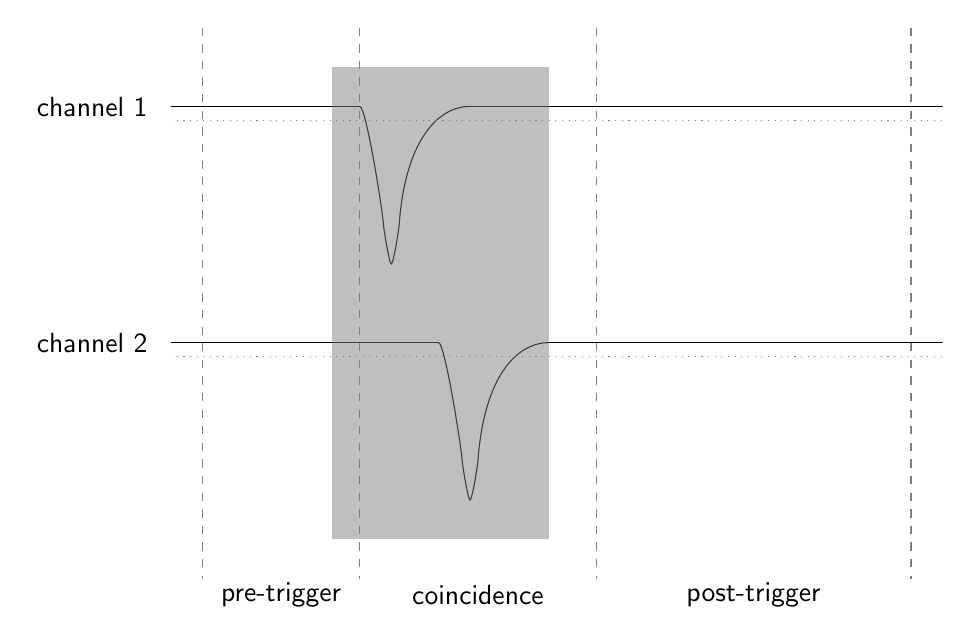
\begin{tikzpicture}[x=2cm,font={\sffamily}]

\node at (-1.7, 0) {channel 1};
\node at (-1.7, -3cm) {channel 2};

\node at (-.5, -6.2) {pre-trigger};
\node at (.75, -6.2) {coincidence};
\node at (2.5, -6.2) {post-trigger};

\clip (-1.2, 1) rectangle (3.7, -6);

\pulse
\begin{scope}[yshift=-3cm,xshift=1cm]
\pulse;
\end{scope}

% Time windows
\draw[gray,dashed] (-1, 1) -- +(0, -7);
\draw[gray,dashed] (0, 1) -- +(0, -7);
\draw[gray,dashed] (1.5, 1) -- +(0, -7);
\draw[gray,dashed] (3.5, 1) -- +(0, -7);

% Reduction Threshold
\draw[gray,dotted] (-1.5, 0 - 5pt) -- +(20, 0);
\draw[gray,dotted,yshift=-3cm] (-1.5, 0 - 5pt) -- +(20, 0);

% Data window
\path[fill,gray,opacity=.5] (0 - 10pt, 0.5) rectangle (2.4cm, -5.5);

\end{tikzpicture}
